%
% TERMINADA, PORFAVOR REVISAR
%

Una aerol\'inea tiene aviones con una capacidad de 90 pasajeros. bas\'andose en informaci\'on hist\'orica un
15\% de los pasajeros que compran el boleto no toman el vuelo (donde se le devuelve el 95\% del valor
del boleto al cliente). Es por esto que la aerol\'inea pone a la venta 103 boletos para un vuelo.

\begin{itemize}
	\item Lea las siguientes preguntas y escriba sus hip\'otesis antes resolver las preguntas.\\
	\item ?`Cu\'al es la cantidad esperada de clientes que tomen el vuelo? ?`Cu\'al es la varianza de clientes que toman el vuelo?\\ \\
	La probabilidad que un pasajero compre un pasaje y tome el vuelo es de $p = 0.85$, por lo que la cantidad esperada de clientes que tomen el vuelo es de:\\
	$E(x) = np = 103*0.85 = 87.55 \approx 88$\\
	La varianza de clientes que toman el vuelo es de:\\
	$V(x) = np(1-p) = 87.55*0.15 = 13.13$\\
	\item ?`Cu\'al es la probabilidad de que un pasajero se quede sin asiento?\\
	Es el complemento de la cantidad de pasajeros que si pueden tomar el vuelo, es decir:\\
	$1 - P(X<=90) = 1 - \sum_{90}^{103} { 103 \choose 90} 0.85^{90} 0.15^{13} = 0.7890807$\\
	\item ?`Cu\'al es la probabilidad de que todos los clientes quieran tomar el vuelo?\\
	Ya que buscamos que los 103 pasajeros que compraron boleto quieran efectivamente tomar el vuelo, se trata de una Binomial de 103 sobre 103, con probabilidad de tomar el vuelo de 0.85, lo cual nos da como resultado $ 5.372165 \cdotp 10^{-8}  $ .\\

	\item Realice gr\'aficos de la funci\'on de densidad de probabilidad y de la funci\'on de distribuci\'on (funci\'on de probabilidad acumulada)\\ \\
	Sea X la cantidad de personas que compran boletos y toman el vuelo, $p = 0.85$, $n = 103$\\
	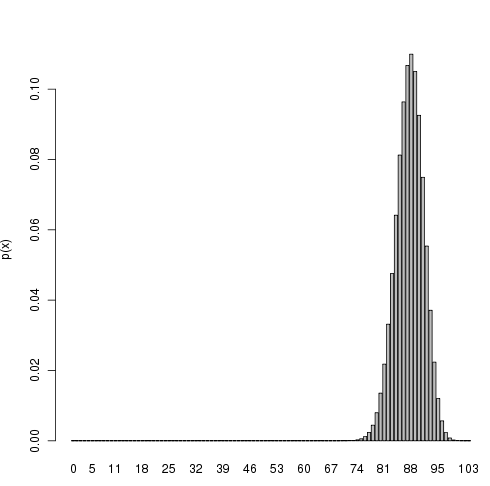
\includegraphics[scale=0.5]{images/1_1-dbinom}\\ %dbinom(x,103,0.85)
	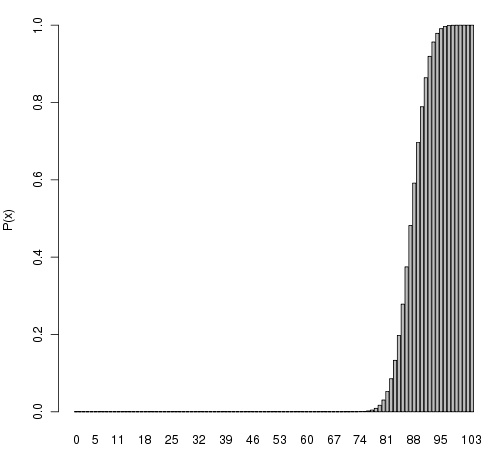
\includegraphics[scale=0.5]{images/1_1-pbinom}\\ %pbinom(x,103,0.85)
	\item Var\'ie el o los valores de los par\'ametros de la distribuci\'on y comente lo observado en los gr\'aficos de la funci\'on de densidad y de distribuci\'on. (2 casos)\\
	\begin{itemize}
		\item Funci\'on de Densidad\\
			En \'esta funci\'on decidimos variar la probabilidad, y nos encontramos con que:\\
			Funcion de Densidad con Probabilidad de 50\% \\
			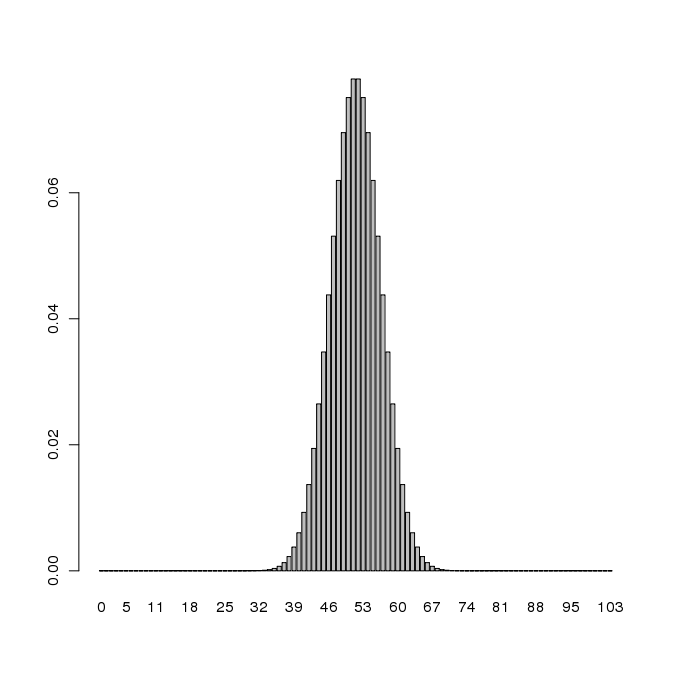
\includegraphics[scale=0.4]{images/1_1-dbinom-prob-variada1}\\
			Funcion de Densidad con Probabilidad de 15\% \\
			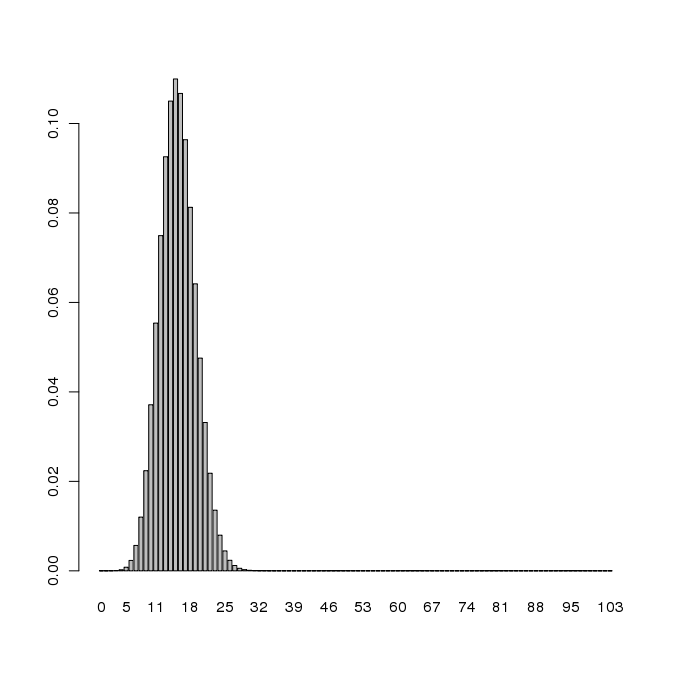
\includegraphics[scale=0.4]{images/1_1-dbinom-prob-variada2}\\
			Como podemos observar, la forma de la densidad se mantiene constante, lo que cambia es la posici\'on con respecto al eje X.\\
		\item Funci\'on de Distribuci\'on\\
			En \'esta funci\'on tambi\'en decidimos variar la probabilidad, y nos encontramos con que:\\
			Funcion de Distribuci\'on con Probabilidad de 50\% \\
			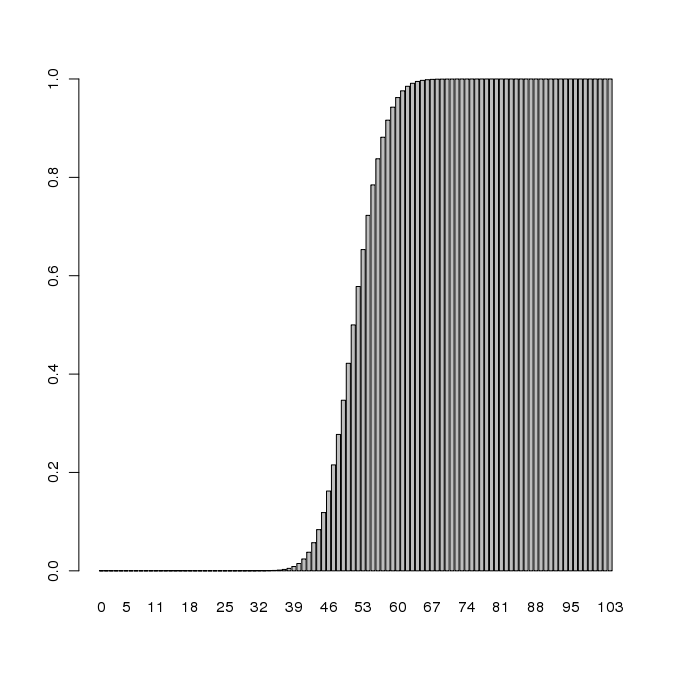
\includegraphics[scale=0.4]{images/1_1-pbinom-prob-variada1}\\
			Funcion de Distribuci\'on con Probabilidad de 15\% \\
                        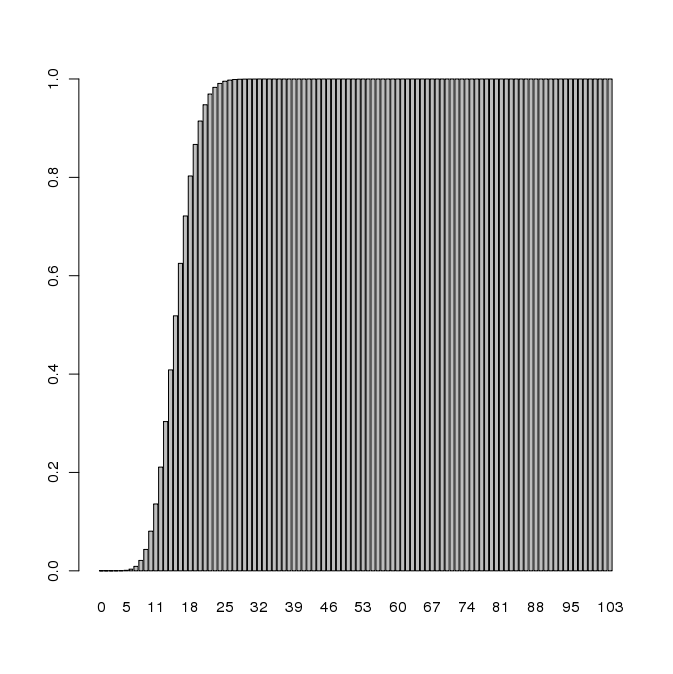
\includegraphics[scale=0.4]{images/1_1-pbinom-prob-variada2}\\
			Como podemos observar, simplemente el comienzo de la acumulada parte cada vez mas atrás mientras vamos disminuyendo la probabilidad.\\

	\end{itemize}

\end{itemize}
